	\indent En el siguiente trabajo práctico se analizará dos esquemas de comunicaciones, uno digital y otro analógico. En ambos casos se transmitirán símbolos que representan 1 bit. Si el bit es 1, el símbolo será A y si es 0 se simbolorizá -A. La probabilidad de que A se 1 o 0 es $\frac{1}{2}$. En cada etapa de estos sistemas de comunicación a la señal se la mutltiplica por un atenuador \emph{h} y se le suma un ruido $W \sim N(0,\sigma ^2)$\\
	
	\indent En el \textbf{repetidor digital}, que se ilustra en la figura \ref{Fig.Sist_dig}, el bloque con la letra \textbf{D} toma una decisión acerca del símbolo transmitido y lo retransmite a la etapa siguiente y es la última etapa donde el detector toma la desición final. La opereación matemática del detector \textbf{D} se puede escribir como:
	
						\begin{equation}
							X_{i+1}=
									\begin{cases}
											A		& \quad \text{si} Y_i \geq 0 \\
											-A		& \quad \text{si} Y_i \leq 0
									\end{cases}
						\label{Eq.sis.digital}
						\end{equation}

	\indent En cambio en el \textbf{repetidor analógico}, cuya representación es la de la Figura \ref{Fig.Sist_ana}, se toma una única decisión y ocurre en el receptor. En los casos intermedios, los símbolos recibidos son multiplicados por una ganancia para luego retransmitirlos a la siguiente estapa. Dichos símbolos se pueden representar según:
	
						\begin{equation}
							x_{I+1} = G_{i+1} \cdot Y_i \quad i=1,....,n-1
							\label{Eq.sis.analogico}
						\end{equation}
						
			\begin{figure}[H]
				\centering
				\begin{subfigure}[b]{0.7\textwidth}
					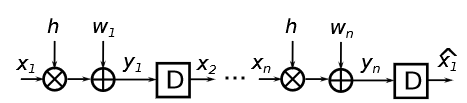
\includegraphics[width=\textwidth]{./Figuras/Sistema_digital}
					\caption{Sistema de comunicación digital}
					\label{Fig.Sist_dig}
				\end{subfigure}
			\begin{subfigure}[b]{0.7\textwidth}
				\includegraphics[width=\textwidth]{./Figuras/Sistema_analogico}
				\caption{Sistema de comunicación analógico}
				\label{Fig.Sist_ana}
			\end{subfigure}
			\caption{Sistemas de comunicaciones con distintos tipos de repetidores}
		\end{figure}